\section{Event Transmission}

The event transmitter is somewhat complex due to the desire to avoid
sending packets with no / few events, but to also avoid event
overflow. A worst-case would be every single event in an event cycle
being directed at the network device; This would result in 960 bytes
of data for the UDP packet. But sending a single event wastes 80% of
the ethernet frame capacity. But we also wish to avoid prolonged
periods of event queuing.

To meet these parameters, we send an event datagram whenever: 
\begin{enumerate}
\item More than 5 ecycles have passed without a transmission
\item we have a buffer whose total length is > 100. 
\end{enumerate} 

\subsection{Implementation}
\begin{figure}
\begin{centering}
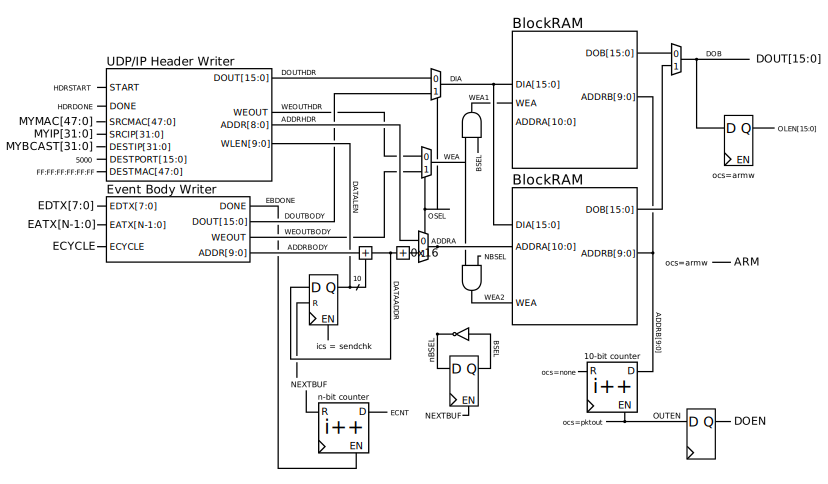
\includegraphics[scale=0.8]{eventtx.svg}
\end{centering}
\caption{Event transmission implementation}
\label{eventtx}
\end{figure}

\begin{figure}
\begin{centering}
\includegraphics[scale=0.8]{eventtx.fsm.svg}
\end{centering}
\caption{Event transmission implementation FSM.}
\label{eventtx.fsm}
\end{figure}

We use two BlockRAM devices to create a double-buffered system where we can acquire new events and transmit old ones simultaneously. Each buffer can hold 2048 bytes, enough for a full-MTU datagram. 

If a buffer has more than 100 bytes of events, say, 105, it's possible that the next ecycle will result in an overflow, so we must transmit. 

At 50 MHz, a 1024-byte event takes 10.3 $\mu s$ to transmit. We need to
maintain the ability for the network TX interface to transmit one of
these per cycle.

Our implementation uses separate FSMs to write the relevant bits for the IP/UDP headers and the. 

\subsection{Event Body Writer}
\begin{figure}
\begin{centering}
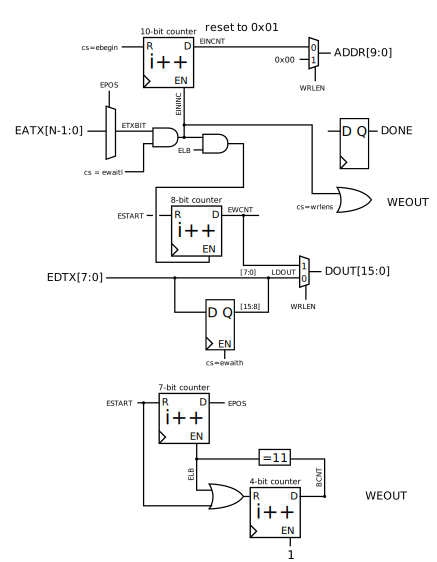
\includegraphics[scale=0.8]{eventtx.eventbody.svg}
\end{centering}
\caption{Event transmission event body writer}
\label{eventtx.eventbody}
\end{figure}

\begin{figure}
\begin{centering}
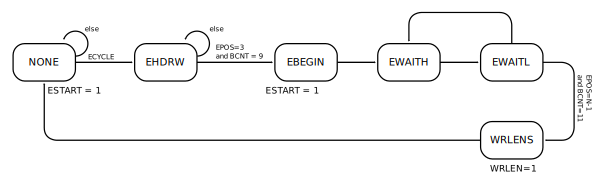
\includegraphics[scale=0.8]{eventtx.eventbody.fsm.svg}
\end{centering}
\caption{Event transmission event body writer}
\label{eventtx.eventbody.fsm}
\end{figure}

The eventbodywriter receives events via an Event Port and: 

1. writes the event data from byte 1 ... 12*N - 1
2. after the events are done, writes the number-of-events-written to byte 0
3. then asserts done. 

We are guaranteed at least 40 ticks between the assertion of ECYCLE
and the first assertion of WEOUT for that cycle. 


At the assertion of DONE, we verify/guarantee that ADDR contains the address of the word that is one-past the last written word. For example, if we wrote one event, then the len was written at addr 0, the event was in 1-12, and ADDR will equal 13 when DONE is asserted, and stay at that for 40 ticks. 

\subsection{Event Header Writer}
The event header writer writes all the unique per-packet data including: 
IP addr
MAC addr
packet length
UDP packet length
frame length
